\documentclass{article}
\usepackage{titlesec}
\usepackage[a4paper, margin=2cm]{geometry}
\usepackage{graphicx}
\titleformat{\section}{\normalfont\Large\bfseries}{\thesection}{1em}{}

\begin{document}

\section*{\textbf{Computer Vision Intermediate Project Report}}

I componenti di questo gruppo ("Gli ultimi Sumiti") sono gli alunni Scantamburlo Mattia, Piai Luca e Chinello Alessandro.  
Nel seguente file abbiamo realizzato un breve report sul progetto svolto, spiegando come ci siamo organizzati, l’idea di base adottata per strutturare il codice, la suddivisione del lavoro, i risultati ottenuti e le principali problematiche incontrate.

\subsection*{Organizzazione della progettazione}
Abbiamo organizzato la nostra pipeline relativa al software per rilevare alcuni oggetti ( quali scatola di zucchero, mostarda e trapano ), in alcune immagini denominate \textit{scene}, secondo la seguente logica:  
\begin{enumerate}
    \item Avendo un dataset specifico per ogni singolo oggetto, contenente immagini che raffigurano prospettive e angolazioni differenti, nella fase iniziale ci siamo concentrati sull’estrazione delle feature da ciascuna categoria del dataset, memorizzandole tramite opportune pratiche. Come algoritmo di rilevazione delle feature ci siamo affidati a SIFT, dopo aver sperimentato diverse alternative, come la combinazione con segmentazione ,SURF, o addirittura approcci completamente diversi come il template matching.

    \item In seguito, abbiamo utilizzato tali dati per eseguire il matching con la scena fornita in input dall’utente, seguendo una procedura sequenziale: data una scena, il software cerca inizialmente la presenza dello zucchero, poi della mostarda e poi del trapano; in caso di rilevamento, viene mostrato un \textit{bounding box} della corrispettiva detection e vengono salvate le relative coordinate (top left e bottom right), secondo le convenzioni delle label del dataset, in un file dedicato. 

    \item Infine, tramite l’elaborazione delle label del dataset, insieme ai dati restituiti dal nostro software, abbiamo calcolato le metriche di valutazione in un file finale, riferito alla scena analizzata. Testando il programma su tutte le scene è stato infine possibile ottenere la mIoU complessiva.
\end{enumerate}

\subsection*{Divisione del lavoro}
Il lavoro è stato  suddiviso in alcune macro aree temporali, che si sono susseguite in maniera sequenziale:
\begin{itemize}
    \item Una prima fase di discussione sull’organizzazione implementativa;
    \item Una fase di sperimentazione, soprattutto per quanto riguarda la rilevazione degli oggetti, durante la quale abbiamo testato varie strategie per individuare quella più efficace, in base ai sample disponibili nel dataset;
    \item Una fase di riunione e briefing in cui siamo passati alla vera e propria strutturazione del codice, suddividendoci lo sviluppo in termini di classi e implementazioni specifiche;
    \item Una fase finale di revisione completa della struttura, con l’introduzione di miglioramenti e modifiche.
\end{itemize}

\subsection*{Problematiche riscontrate}
Le principali difficoltà sono emerse nella seconda fase, in cui ci siamo “dispersi” nel tentativo di individuare l’approccio migliore. Qualunque direzione prendessimo in termini di matching con le scene reali, non siamo mai riusciti a ritenerci pienamente soddisfatti. Probabilmente ciò è dipeso anche dal numero limitato di sample per ciascun oggetto nel dataset.

\subsection*{Risultati}



 


\begin{figure}[H]
  \centering
  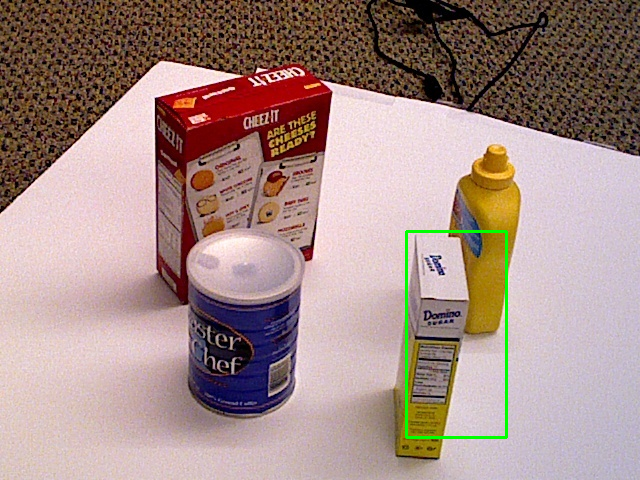
\includegraphics[width=0.48\textwidth]{immagine1.jpg} % Prima immagine (modifica il nome)
  \hfill
  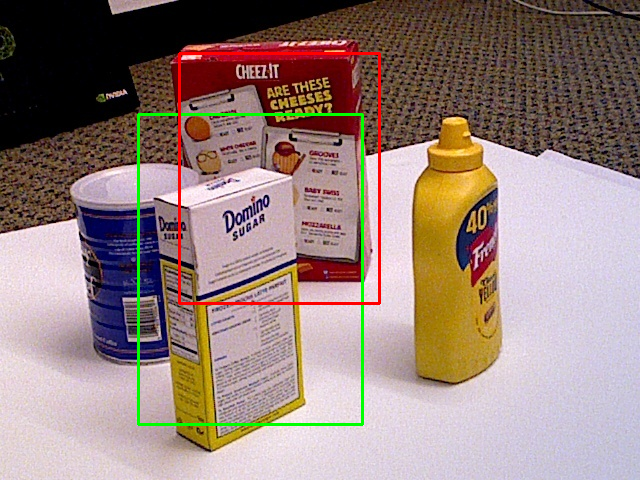
\includegraphics[width=0.48\textwidth]{immagine2.jpg} % Seconda immagine (modifica il nome)
\end{figure}

\begin{figure}[H]
  \centering
  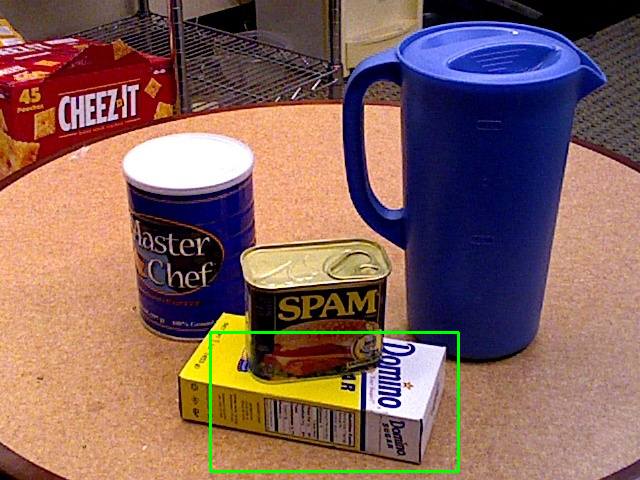
\includegraphics[width=0.48\textwidth]{immagine3.jpg}
  \hfill
  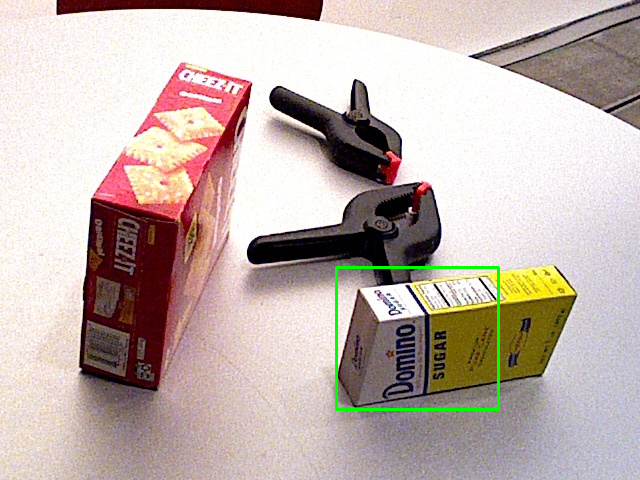
\includegraphics[width=0.48\textwidth]{immagine4.jpg}
\end{figure}

\begin{figure}[H]
  \centering
  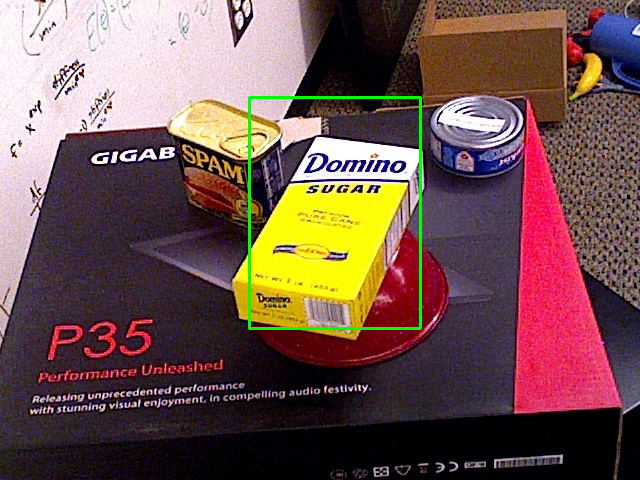
\includegraphics[width=0.48\textwidth]{immagine5.jpg}
  \hfill
  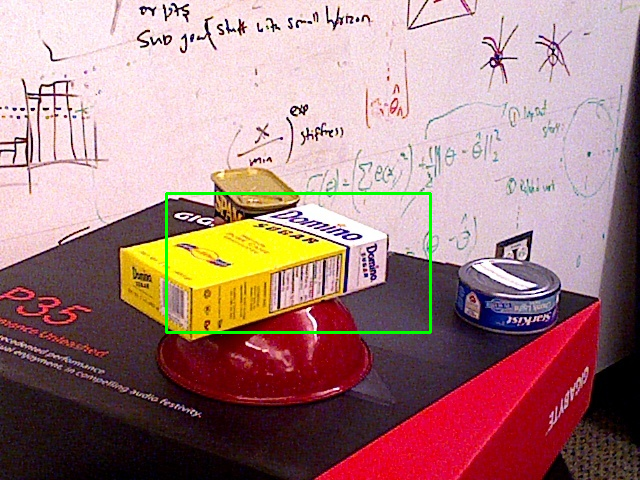
\includegraphics[width=0.48\textwidth]{immagine6.jpg}
\end{figure}

\begin{figure}[H]
  \centering
  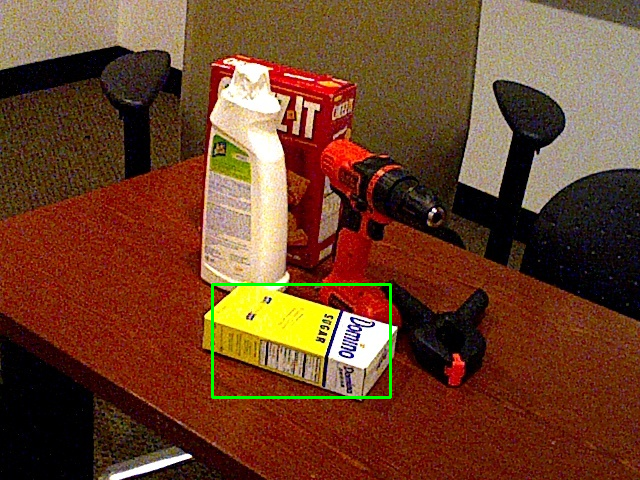
\includegraphics[width=0.48\textwidth]{immagine7.jpg}
  \hfill
  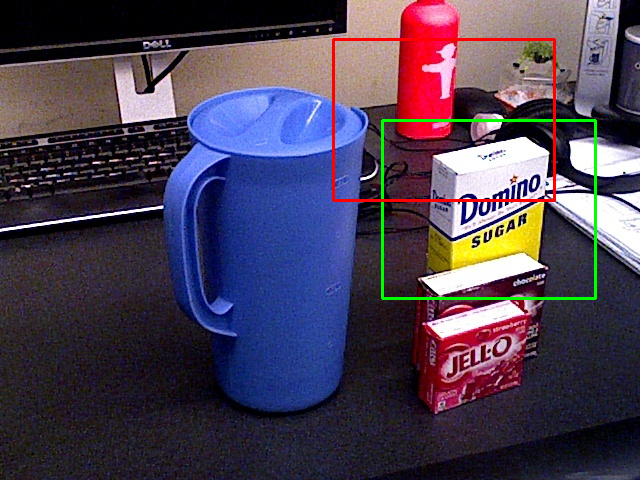
\includegraphics[width=0.48\textwidth]{immagine8.jpg}
\end{figure}

\begin{figure}[H]
  \centering
  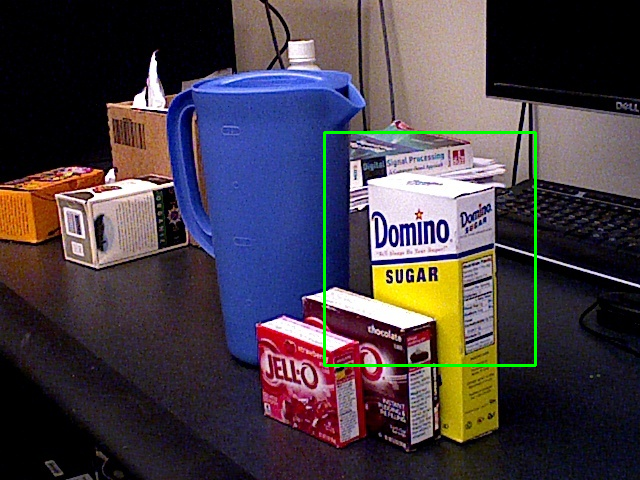
\includegraphics[width=0.48\textwidth]{immagine9.jpg}
  \hfill
  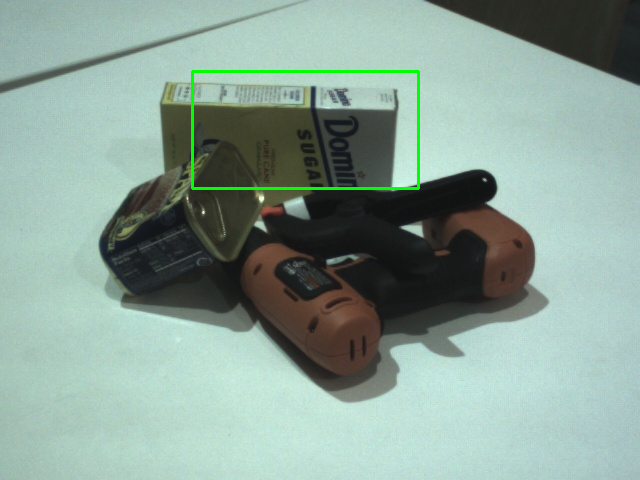
\includegraphics[width=0.48\textwidth]{immagine10.jpg}
\end{figure}

\begin{figure}[H]
  \centering
  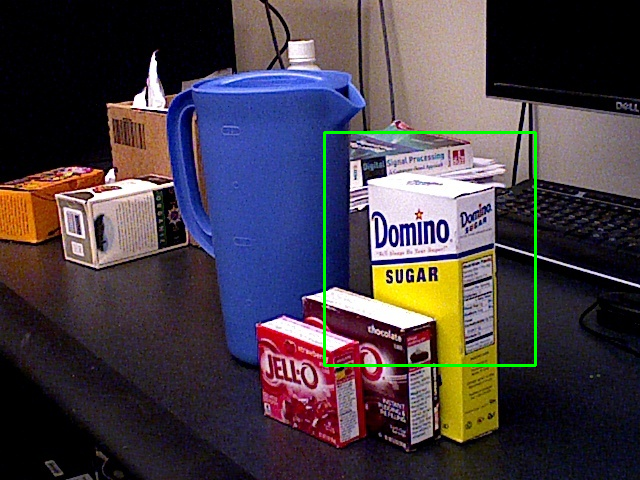
\includegraphics[width=0.48\textwidth]{immagine9.jpg}
  \hfill
  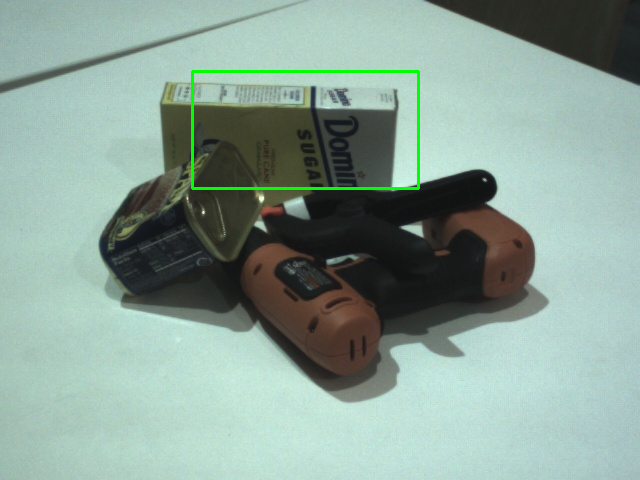
\includegraphics[width=0.48\textwidth]{immagine10.jpg}
\end{figure}


\end{document}
